% Template for PLoS
% Version 3.1 February 2015
%
% To compile to pdf, run:
% latex plos.template
% bibtex plos.template
% latex plos.template
% latex plos.template
% dvipdf plos.template
%
% % % % % % % % % % % % % % % % % % % % % %
%
% -- IMPORTANT NOTE
%
% This template contains comments intended 
% to minimize problems and delays during our production 
% process. Please follow the template instructions
% whenever possible.
%
% % % % % % % % % % % % % % % % % % % % % % % 
%
% Once your paper is accepted for publication, 
% PLEASE REMOVE ALL TRACKED CHANGES in this file and leave only
% the final text of your manuscript.
%
% There are no restrictions on package use within the LaTeX files except that 
% no packages listed in the template may be deleted.
%
% Please do not include colors or graphics in the text.
%
% Please do not create a heading level below \subsection. For 3rd level headings, use \paragraph{}.
%
% % % % % % % % % % % % % % % % % % % % % % %
%
% -- FIGURES AND TABLES
%
% Please include tables/figure captions directly after the paragraph where they are first cited in the text.
%
% DO NOT INCLUDE GRAPHICS IN YOUR MANUSCRIPT
% - Figures should be uploaded separately from your manuscript file. 
% - Figures generated using LaTeX should be extracted and removed from the PDF before submission. 
% - Figures containing multiple panels/subfigures must be combined into one image file before submission.
% For figure citations, please use "Fig." instead of "Figure".
% See http://www.plosone.org/static/figureGuidelines for PLOS figure guidelines.
%
% Tables should be cell-based and may not contain:
% - tabs/spacing/line breaks within cells to alter layout or alignment
% - vertically-merged cells (no tabular environments within tabular environments, do not use \multirow)
% - colors, shading, or graphic objects
% See http://www.plosone.org/static/figureGuidelines#tables for table guidelines.
%
% For tables that exceed the width of the text column, use the adjustwidth environment as illustrated in the example table in text below.
%
% % % % % % % % % % % % % % % % % % % % % % % %
%
% -- EQUATIONS, MATH SYMBOLS, SUBSCRIPTS, AND SUPERSCRIPTS
%
% IMPORTANT
% Below are a few tips to help format your equations and other special characters according to our specifications. For more tips to help reduce the possibility of formatting errors during conversion, please see our LaTeX guidelines at http://www.plosone.org/static/latexGuidelines
%
% Please be sure to include all portions of an equation in the math environment.
%
% Do not include text that is not math in the math environment. For example, CO2 will be CO\textsubscript{2}.
%
% Please add line breaks to long display equations when possible in order to fit size of the column. 
%
% For inline equations, please do not include punctuation (commas, etc) within the math environment unless this is part of the equation.
%
% % % % % % % % % % % % % % % % % % % % % % % % 
%
% Please contact latex@plos.org with any questions.
%
% % % % % % % % % % % % % % % % % % % % % % % %

\documentclass[10pt,letterpaper]{article}
\usepackage[top=0.85in,left=2.75in,footskip=0.75in]{geometry}
\usepackage{changes}


% Added for vertically merged cells in table header
\usepackage{multirow}

% Use adjustwidth environment to exceed column width (see example table in text)
\usepackage{changepage}

% Use Unicode characters when possible
\usepackage[utf8]{inputenc}

% textcomp package and marvosym package for additional characters
\usepackage{textcomp,marvosym}

% fixltx2e package for \textsubscript
\usepackage{fixltx2e}

% amsmath and amssymb packages, useful for mathematical formulas and symbols
\usepackage{amsmath,amssymb}

% cite package, to clean up citations in the main text. Do not remove.
\usepackage{cite}

% Use nameref to cite supporting information files (see Supporting Information section for more info)
\usepackage{nameref,hyperref}

% line numbers
\usepackage[right]{lineno}

% ligatures disabled
\usepackage{microtype}
\DisableLigatures[f]{encoding = *, family = * }

% rotating package for sideways tables
\usepackage{rotating}

% Remove comment for double spacing
%\usepackage{setspace} 
%\doublespacing

% Text layout
\raggedright
\setlength{\parindent}{0.5cm}
\textwidth 5.25in 
\textheight 8.75in

% Bold the 'Figure #' in the caption and separate it from the title/caption with a period
% Captions will be left justified
\usepackage[aboveskip=1pt,labelfont=bf,labelsep=period,justification=raggedright,singlelinecheck=off]{caption}

% Use the PLoS provided BiBTeX style
\bibliographystyle{plos2015}

% Remove brackets from numbering in List of References
\makeatletter
\renewcommand{\@biblabel}[1]{\quad#1.}
\makeatother

% Leave date blank
\date{}

% Header and Footer with logo
\usepackage{lastpage,fancyhdr,graphicx}
\usepackage{epstopdf}
\pagestyle{myheadings}
\pagestyle{fancy}
\fancyhf{}
\lhead{
\includegraphics[width=2.0in]{PLOS-submission.eps}}
\rfoot{\thepage/\pageref{LastPage}}
\renewcommand{\footrule}{\hrule height 2pt \vspace{2mm}}
\fancyheadoffset[L]{2.25in}
\fancyfootoffset[L]{2.25in}
\lfoot{\sf PLOS}

%% Include all macros below

\newcommand{\lorem}{{\bf LOREM}}
\newcommand{\ipsum}{{\bf IPSUM}}

%% END MACROS SECTION


\begin{document}
\vspace*{0.35in}

% Title must be 250 characters or less.
% Please capitalize all terms in the title except conjunctions, prepositions, and articles.
\begin{flushleft}
{\Large
% \textbf\newline{The sonic instructor: a music biofeedback system for improving weightlifting technique}
\textbf\newline{The sonic instructor: a music-based biofeedback system for improving weightlifting technique}
}
\newline
% Insert author names, affiliations and corresponding author email (do not include titles, positions, or degrees).
\\
Valerio Lorenzoni\textsuperscript{1,*},
Jacob Staley\textsuperscript{2},
Kelsey Onderdijk\textsuperscript{1},
Marc Leman\textsuperscript{1}

\bigskip

\textbf{1} Institute for Psychoacoustics and Electronic Music (IPEM), Department of Musicology, Ghent University, Ghent, Belgium
\\
\textbf{2}  Internet technology and data science lab (IDLAB), Ghent University, Ghent, Belgium
%\\
%\textbf{3} Data analysis Department, Ghent University, Ghent, Belgium
\\

\bigskip



 %Use the asterisk to denote corresponding authorship and provide email address in note below.
* valerio.lorenzoni@ugent.be

\end{flushleft}
% Please keep the abstract below 300 words

\section*{Abstract}

Crossfit and gymnastic exercising are becoming increasingly popular. Functional movement are the the base of such exercises and 

usually these kind of movement require specific technique for movement improvement and 


\section*{Introduction}

Biofeedbacks have been used for over fifty years in the domains of sports \cite{onate2001augmented} and motor rehabilitation \cite{tate2016real} . These techniques are used to provide the subjects with information about physiological or biomechanical parameters that that would otherwise be unknown.
\cite{giggins2013biofeedback}. 

%Many physiological processes that directly influence our physical and cognitive performance are not under our conscious control. Biofeedbacks offer a possibility to monitor and correct 

The main goal of such systems is to let the subject automatically improve the performances at subconscious level, without explicit instructions by a trainer or therapist.
Traditionally biofeedback are presented to the subject via visual displays , acoustic or vibrotactile feedback. Recent technological developments have opened the possibility to provide such bio-feedback in real-time during physical activity, this opened the possibility for using
A recent development in rehabilitation is exercising in a gaming or virtual reality (VR) environment, thus providing a novel form of immersive biofeedback.

In this paper we describe the design and validation process of a bio-mechanical biofeedback system for improving weightlifting movements.


Weightlifting is an ancient sport which appeared in the Olympic Games in Athens already in 1896. Weightlifting movements are becoming increasingly popular in the sport world, as new sports as Crossfit (founded in year 2000 by) combine elements of Olympic weight lifting together with other disciplines.
Although researchers have proven the benefits of such functional weightlifting movements \cite{smith2013crossfit}, deep knowledge of the exact technique is required in order to maximize movement efficency and minimize the chance of injuries.

In this work we focused on a specific movement called \emph{deadlift} which one of the three discipline of power lifting movements but it is widely used in weightlifting training and rehabilitation practices.

According to the handbook of the powerlifting federation \cite{} a deadlift consists of grabbing a barbell from the floor with hands, then raising the weight by extending the knee, hips, and back while holding the arms downward. On completion of the lift, the knees must be locked in a straight position adn the shoulders pulled back.

McCuigan \emph{et al.} investigated the kinematics of deadlift comparing different techniques: the Sumo and conventional style.

Due to the fact that the DL is a closed chain exercise [5], it is often used in the prevention of and rehabilitation after anterior cruciate ligament (ACL) reconstruction to improve strength of the muscular structures that surround the knee and hence dynamic stability of the joint 

However, a wrong technique during deadlift lift-off may predispose the spine and back musculature to an increased risk of injury \cite{granhed1987loads,cholewicki1991lumbar}. The exercise is often made unsafe by the lifter rounding his back and bending over too far at the hips just before lifting. Holding the bar away from your body instead of right against it is another way to injure your back. At the top of the movement, avoid hyperextending your lower back. Some people lean back a little at the top, but doing so only asks for trouble.


With the presented system we aim at providing a real-time feedback using auditory displays, i.e. sonification. The quantities to be sonified and on which the participant gets feedback are the spine curvature and the barbell horizontal displacement as these quantities are directly related to back loads and injuries.

Usually coaches spend time in the first phase to teach the right technique and provide feedbacks to the performers.

Having continuous feedback by a coach is not feasible while training in public gyms or at home. Therefore there is need to develop portable systems able to guide towards the right movement technique.


The use of sonification in weightlifting has been shown to increase average exertion of power in the experimental condition, compared to the control condition. \cite{murgia2012using}. The work of







Apart from learning the technique the system could be used for advanced sporters to further improve their technique by discovering minor aspects of their movement that are not fully visible by eye.



We measured the power exerted during the lifting. The results show that athletes can take advantage of the stimulus we provided, evidencing a higher average exertion of power in the experimental condition, compared to the control condition. Concluding, the results suggest that auditory perception can be a productive field of research in developing experimental strategies to improve athletes? skills.




Our hypothesis is that such system could be comparable to the verbal instructions by and instructor in terms of performances and that would be more motivating than standard verbal instruction because of the reward mechanism.



% FROM PIETER-JAN JMUI
In the domain of sports and motor rehabilitation, sonification of physical and physiological data is typically used to serve three functions, namely to motivate, to monitor, and/or to modify human performance. Auditory feedback has been proven particularly useful in assisting motor learning and adaptation. The way sonification, or auditory biofeedback, is deployed for this purpose may rely on different strategies. The most typical strategy pertains to a goal-driven approach. This approach requires that the learner has an explicit representation of the target behavior, i.e., the goal. Sonification then functions as mere information carrier, allowing people to monitor their behavior, compare it to the target behavior, and adapt their behavior if required [2?4]. 

As indicated by Ram and Leake [5], this process is guided by reasoning and attention mechanisms and may therefore not always be the most appropriate strategy. Recently, a promising alternative strategy is being explored, drawing upon basic principles from the reinforcement learning paradigm. Reinforcement learning is rooted in the idea that people act and behave so as to maximize outcome reward. Hence, when coupling a reward to a desired behavior, people are likely to exhibit this behavior spontaneously, without needing to be told explicitly what to do. In this context, music and sound are particularly relevant as they might be rich sources of reward and pleasure (for an in-depth discussion, see [1])

Music is of particular interest for sonification because many humans are highly skilled in synchronizing temporal and spatial aspects of their move- ments to parameters in the sound and music. The periodic character of the music (implied in the expressive timing of pulses and beats) fits well with the ability of the human motor system to act in concert with attention sharpened by period- icity in signals [29], as music is often designed to dance and move upon [40]. On top of that, a major asset of using music as feedback source concerns its ability to motivate and provide pleasure [32]. This feature may be related to its rhythmicity [40], which is valuable in contexts that often involve strenuous physical activity, boredom, and fatigue [11].




\section*{Materials and Methods} \label{sec:materials_methods}
\subsection*{Ethics statement}
The study was approved by the Ethics Committee of the Faculty of Arts and Philosophy of Ghent University, and all procedures followed were in accordance with the statements of the Declaration of Helsinki. All participants voluntarily participated; They were informed about the physical effort required for the experiment and that questionnaires could have contained personal questions.

\subsection*{Participants}
Participants consisted of 28 non-professional weightlifters with an average age of 24 $\pm$ 5 years. 

The distribution between sexes was relatively even with 46\% women and 54\% men. 61\% of the participants had music education. Most of them (82\%) were educated in an academy, 12\% was self-educated and 6\% took private lessons. A majority of 86\% went jogging at least once a month. The exact numbers are: 21\% once a month, 25\% once a week and 52\% several times a week. 

\subsection*{Apparatus}\label{sec:apparatus}
Experiments took place a the 
Participants were equipped with a full body MOCAP markers set-up
\begin{figure}[!h]
\center
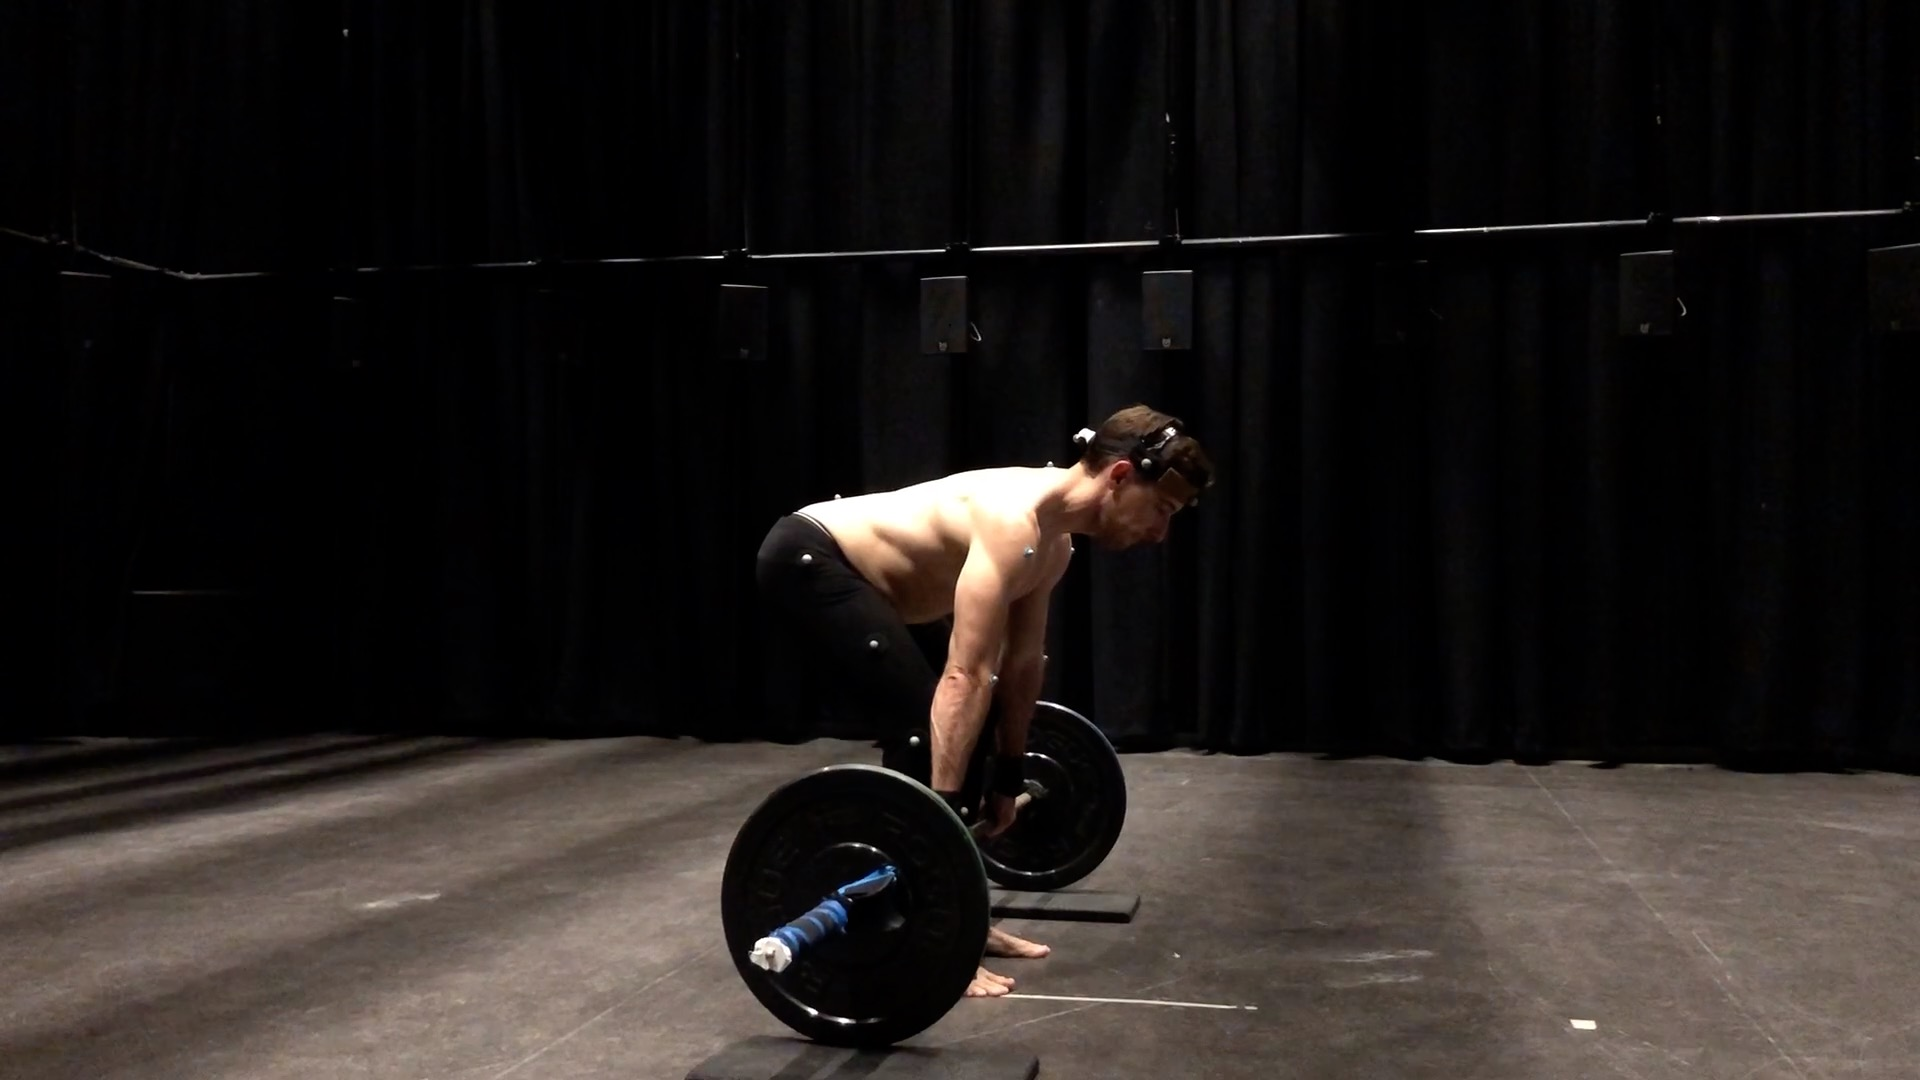
\includegraphics[width=.8\textwidth]{figures/promo1_deadlift.jpg}
\caption{Sketch experimental set-up}
\label{fig:set-up}      
\end{figure}

\subsection*{Experimental procedure}
Participants were asked to perform 10 repetitions in 


\begin{figure}[!h]
\center
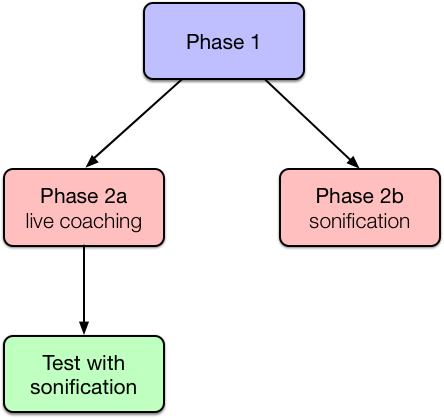
\includegraphics[width=.8\textwidth]{figures/Experiment-flow.png}
\caption{Experiment workflow}
\label{fig:workflow}      
\end{figure}


The 3 points of performance consisted of :
\begin{enumerate} %for small alpha-characters within brackets.
\item  \emph{Spine}: a reference condition without music, 
\item  \emph{Barbell}: an adaptive BPM and phase synchronization based on the DJogger technology \cite{moens2014encouraging}
\item  \emph{Combination}: a tempo synchronization condition based on the initial SPM of the runner
\end{enumerate}



After each run, a break of 5 minutes was introduced to enable the participant to recover sufficiently. During the break they were asked to fill out a Rating of Perceived Exertion (RPE) questionnaire \cite{borg1998borg} and indicate how heavy the effort had been during the exercise, ranging from 6 ("no exertion at all") to 20 ("maximal exertion"). In addition, they rated the level of physical enjoyment of the previous run on the 8-item version of the Physical Activity Enjoyment Scale (PACES) \cite{kendzierski1991physical}, a single factor scale to assess the level of enjoyment during a physical activity in adults across exercise modalities.
In order to test the motivational properties of the stimulus, participants also performed a modified version of the Brunel Music Rating Inventory 2 (BMRI-2) test \cite{karageorghis2006redesign}. In this test, they were asked to rate pleasantness and motivational aspects of the music synchronization strategy. They also filled out a questionnaire on music education and sports training. 

%It was also checked whether participants believed they had entrained their running movements with the music in the instructed condition and whether they believe they tend to do so in daily live (in case they run to music).
 

\subsection*{Stimuli}


In all conditions the same music piece was played. The piece was specifically composed for this experiment by Myrthe van de Weetering.\footnote{www.myrthevandeweetering.com}
The music was composed respecting the following requirements:
\begin{itemize}
\item to be unknown, to avoid personal affection
\item to be instrumental (no lyrics), to avoid focus on content
\item to have a clear beat, in order to highlight the difference between synchronized and non-synchronized conditions.
\end{itemize}


\subsection*{Data acquisition}
For each condition the 3D accelerations measured by the accelerometers, were converted into resultant non-dimensional g-force. Cadence (SPM) was also calculated by the JAVA software (through a moving average over 5 steps) and locally stored on the tablet, together with the speed measurements from the sonar. 
The g-force and SPM were continuously transmitted as OSC to an in-house MAX/MSP program running on the same tablet, which implemented the synchronization strategies and provided the audio. Data were collected every detected step and stored as .txt file on the tablet.f

\subsection*{Data analysis}

A preliminary analysis of normality of the data 

t-test 


speak of power as the probability of not making a beta, or a "Type II" error, which refers to falsely concluding that there was no difference (e.g., between experimental and control groups) when in fact there was a difference, but the study failed to show it.

\section*{Results} \label{sec:results}



\subsection*{Differences in performance between feedbacks}


\paragraph{Spine bending differences}

\begin{figure}[!h]
\center
  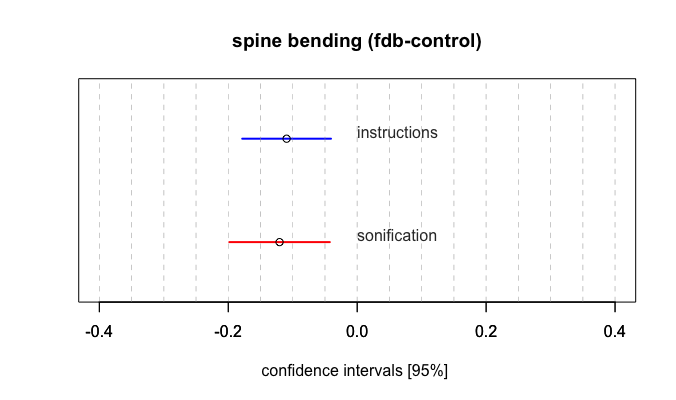
\includegraphics[width=.5\textwidth]{figures/CI_spine_bending.png} 
  \caption{Differences between the instruction and sonification feedbacks} 
  \label{fig:boxplot}      
\end{figure}


\begin{figure}[!ht] 
    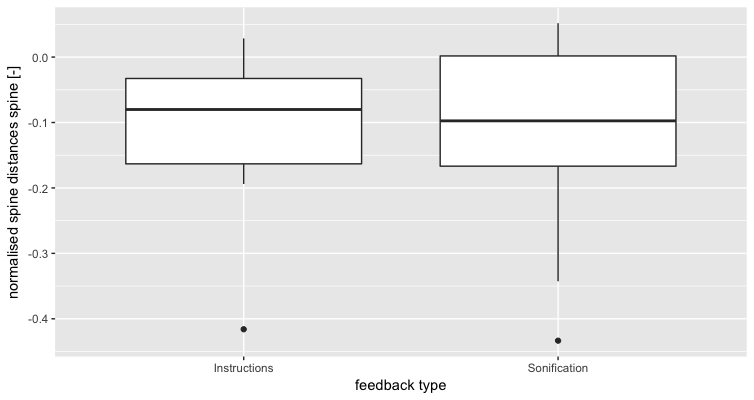
\includegraphics[width=.45\textwidth]{figures/boxplot.png}
\caption{boxplot between 2 feedbaccks}
\label{fig:boxplot} 
\end{figure}


\paragraph{Barbell verticality}








\subsection*{Pairwise differences}



A KS-test for normality revealed that g differences for Adaptive sync condition were normally distributed ($p=0.06$) as well as for the  Plus 30\% ($p=0.2$). The conditions Initial sync ($p=0.022$), Minus 30\% ($p=0.016$) and No music ($p=0.001$) were not normally distributed. 
Paired t-tests were performed on the normally distributed pairs, Wilcoxon tests on the non-normally distributed ones. A summary of the results is shown in Table \ref{tab:parwise} with effect size Cohen $d$ for t-tests and Pearson correlation coefficient $r$ for Wilcoxon tests:




\subsection*{Questionnaires information}

Participants were asked to rate pleasantness and motivational effect of the different synchronisation strategies on a 7-point Likert scale. No overall significant difference was found across conditions using a non parametric Friedman test ($p > 0.05$). 

When comparing independent groups by means of Mann Whitney tests, differences in pleasantness ratings were observed between participants with music education (17) and participants without music education (11) for some of the experimental conditions.
The results are presented in Table \ref{tab:table1}.
%Ratings for each condition were compared among independent groups: participants with music education and participants without by means of Mann Whitney tests.

\begin{table}[h!]
  \begin{center}
    \caption{Results of Mann-Whitney tests on pleasantness ratings}
    \label{tab:table1}
    \begin{tabular}{|c|c|c|c|c|}
    \hline
      \textbf{Condition} & \textbf{Music} & \textbf{No music} & \textbf{z} & \textbf{p}\\
          & \textbf{education (Mdn)} & \textbf{education (Mdn)} & & \\
         \hline
      Adaptive Synch & 5 & 4 & -2.598 & \textbf{0.013} \\     
      Initial Synch & 5 & 5 & -1.620 & $>0.05$\\     
      Minus 30\% & 5 & 4 & -1.615 & $>0.05$\\     
      Plus 30\% & 5 & 4 & -2.244 & \textbf{0.029} \\   
      \hline
    \end{tabular}
  \end{center}
\end{table}






No significant differences were found across gender and across training level of participants. 

\section*{Discussion} \label{sec:discussion}

In this case no effect of arousal produced by the acoustic stimulus was noticed compared to the no sonification condition. E certo se era distorsion!!




Portability of the system could be improved by adoption of current systems for back posture detection ViPerform tm Assessment Modules


Our hypothesis was is that such system could be comparable to the verbal instructions by and instructor in terms of performnces 

However no significant differences were found between the two feedbackss across participants in terms of pleasantness and motivational qualities: reasons could be

choice of music (elaborate)
people used to having a coach
people prefer human feedback






%The design of sonification strategies has been largely investigated for runners gait parameters modifications \cite{bank2011comparing}

\subsection*{Conclusions}

An experiment was performed to check the influence of different music synchronisation strategies on runner's foot strike impact. From the analysis, synchronisation seems not to lead to variations in impact level. However, music onset seems to cause an average impact level increase of 17\% compared to running without music, irrespective of the synchronisation strategy.
No significant difference in pleasantness and motivational effect were observed across the different synchronisation strategies, although phase alignment of the footfalls with music beats seems to be preferred by people with musical background. 



\section*{Acknowledgments}
The authors would like to thank the students of the course Sysmus2017 for the help carrying out the experiments. Bruno De Wannemaeker and the staff of the Topsport Hall in Gent is also gratefully acknowledged for their availability and support during the tests.
\nolinenumbers

%\section*{References}
% Either type in your references using
% \begin{thebibliography}{}
% \bibitem{}
% Text
% \end{thebibliography}
%
% OR
%
% Compile your BiBTeX database using our plos2015.bst
% style file and paste the contents of your .bbl file
% here.
% 

\bibliographystyle{plos2015}
\bibliography{/Users/valerioipem/Dropbox/MyIPEM/Publications/IPEMBibliography}


\end{document}


